\section{Uncertainty}\index{Uncertainty}
A purely logical approach may not work very well for statements which include multiple uncertain factors(e.g. Road accident on your way to the airport? Road work? Flooding? Nazi Zombies?\\
A purely logical approach would state: "$A_8$ will get me there on time."\\
Considering uncertain factors this would change to:"If there's no accident on the bridge, and it does not rain, and my tires remain intact etc, THEN $A_8$ will get me there on time"\\

Reasons for that:\\
\begin{itemize}
\item Failure to enumerate exceptions, qualifications etc.
\item No complete theory for the domain
\item Lack of relevant facts, initial conditions and so on
\end{itemize}

\subsection{Probability for handling uncertainty}
Probabilistic provides a way of summarizing the uncertainty.\\
An example for that would be: conditional probabilities can be used to represent:\\
\begin{itemize}
\item Given the available evidence, $A_8$ will get me there on time with probability 0.8
\item Given the available evidence, $A_10$ will get me there on time with probability 0.9
\item Given the available evidence, $A_12$ will get me there on time with probability 0.99
\end{itemize}

\begin{table}[h]
\centering
\begin{tabular}{l|l|l}
\toprule
\textbf{Condition} & \textbf{Result} & \textbf{Probability}\\
\midrule
Given the available evidence & $A_8$ & 0.9 \\
Given the available evidence & $A_10$ & 0.99\\
Given the available evidence & $A_12$ & 0.999\\
\bottomrule
\end{tabular}
\caption{Table representation of the different plans}
\end{table}

Probability theory is a main tool for dealing with degrees of belief.\\

\subsubsection{Making decisions}
Suppose given the following statements:\\

\begin{table}[h]
\centering
\begin{tabular}{l l}
P($A_8$  gets me there on time | Condition = & 0.9\\
P($A_{10}$ gets me there on time | Condition = & 0.99\\
P($A_{12}$ gets me there on time | Condition = & 0.999\\
P($A_{24}$ gets me there on time | Condition = & 0.9999\\
\end{tabular}
\end{table}

Given that, what actions to choose?\\
\begin{itemize}
\item Depends on preferences, e.g. the length of the wait at the airport
\end{itemize}

Utility theory is used to represent and infer preferences.\\
Decision theory = utility theory + probability theory\\

\section{Probability}
Subjective or Bayesian probability:\\

\begin{itemize}
\item Probabilities relate propositions to one's own state of knowledge, e.g. $P(A_8 | no reported accidents) = 0.9$
\item But might be learned from past experience from past experiences of similar situations
\item Probabilities of propositions change with new evidence: e.g. $P(A_8|no reported accidents, leave at 5 am) = 0.95$
\end{itemize}

Sample point:\\
A set $Omega $- the sample space: $\omega \in \Omega$ is a sample point or atomic event, e.g. 6 possible rolls of a dice.\\
A probability model/space is a sample space with assigning a probability for every $\omega \in \Omega$ 

\begin{itemize}
\item $P(1) = P(2) = P(3) = P(4) = P(5) = P(6) = 1/6$
\item Property: $0 \leq P(\omega) \leq 1 $ for every $\omega \in \Omega$, $\sum_{\omega \in \Omega} P(\omega) = 1$
\end{itemize}

\subsection{Event}
An event \textit{A} is any subset of $\Omega$.\\

\begin{equation}
P(A) = \sigma_{\omega \in A}P(\omega)
\end{equation}

\begin{itemize}
\item An event is 'dice roll is less than 4'
\item The probability of the event happening is $P(dice roll < 4)=P(1)+P(2)+P(3)=1/2$
\end{itemize}

In AI's language, the sets are decribed by propositions:
\begin{itemize}
\item $\phi$ is "dice roll is less than 4" 
\item $P(\phi) = \Sigma_{\omega \in \phi} P(\omega)$
\end{itemize}

\subsection{Random variables}
A random variable $X:\Omega \rightarrow R$ is a function from sample points to some range, e.g., the reals or Boolean.\\
Let $X(\omega)$ be a Boolean variable to represent whether a dicing result $\omega$ is odd, then:\\  

$X(1) = true$\\
$X(2) = False$\\

But usually written in short \textit{Odd} $P(Odd)$

\subsection{Probability Distribution}
For a random variable \textit{X} taking values from $x_1, \dots, x_k$ probability distribution $P(X = x_i)$ is the probability of \textit{X} taking the value of $x_i$:\\

\begin{table}[h]
\centering
\begin{tabular}{l l l}
$P(odd = true)$ & = & $P(1) + P(3) + P(5)$ \\
 & = & $1/6 + 1/6 + 1/6$ \\
 & = & $1/2$ \\
 $P(Odd = false)$ & = & $P(2) + P(4) + P(6)$ \\
 & = & $1/6 + 1/6 + 1/6$\\
 & = & $1/2$
\end{tabular}
\end{table}

\subsection{Prior probability}
Prior or unconditional probabilities refer to degrees of belief in propositions in the absence of any other information\\

\begin{itemize}
\item $P(Cavity = true) = 0.1$
\item $P(Weather = Sunny) = 0.72$
\end{itemize}

Probability distribution gives values for all possible probabilities:\\
$P(Weather) = <0.72, 0.1, 0.08, 0.1> $normalized, i.e. sums to 1.\\

\begin{table}[h]
\centering
\begin{tabular}{l l}
$P(Weather = sunny)$ & = 0.72\\
$P(Weather = rain)$ & = 0.1\\
$P(Weather = cloudy)$ & = 0.08\\
$P(Weather = snow)$ & = 0.1
\end{tabular}
\end{table}

\subsection{Joint Probability distribution}
Joint Probability distribution for a set of r.v.s gives the probability of every atomic event on those r.v.s(i.e. every sample point)\\

\begin{table}[h]
\centering
\begin{tabular}{|l|l|l|l|l|}
\toprule
 & \multicolumn{2}{ |c| }{Toothache} &\multicolumn{2}{ |c| }{$\neg$ Toothache}\\
 \hline
 & catch & $\neg$catch & catch & $\neq$ catch\\ 
\midrule
 cavity & 0.108 & 0.012 & 0.072 & 0.008\\
 \hline
 $\neg$cavity & 0.016 & 0.064 & 0.144 & 0.576 \\
 \bottomrule
\end{tabular}
\end{table}

\subsection{Conditional probability}
Conditional or posterior probabilities: \\
given some information, sometimes called evidence, the probability of an event happening under the evidence.

\begin{itemize}
\item If a patient is observed to have toothache and no other information is yet available, then the probability of having cavity is 0.8
\item P(cavity|tootache) = 0.8
\end{itemize}

\begin{equation}
Tootache = true \Rightarrow P(cavity|tootache) = 0.8
\end{equation}


If we know more facts e.g. cavity is also given, then we have:\\
$P(cavity|tootache, cavity) = 1$
The less specific belief \textit{remains valid} after more evidence arrives, but is not always \textit{useful}. New evidence may be irrelevant, allowing simplification, e.g.:\\
\begin{equation}
P(cavity|tootache, dice = 1) = P(cavity|tootache) = 0.8
\end{equation}


This kind of inference, sanctioned by domain knowledge, is crucial.

\begin{theorem}[Definition of conditional probability]
\begin{align}
P(a|b) = \frac{P(a \cap b)}{P(b)} if P(b) \neq 0
\end{align}
\end{theorem}

When the example used so far is applied to this theorem we will get this:\\
\begin{equation}
P(cavity|tootache) = \frac{P(cavity, foothache}{P(tootache)}
\end{equation}

If the product rule is applied, it gives an alternative formulation:\\
\begin{equation}
P(a \cap b) = P(a|b)P(b) = P(b|a)P(a)
\end{equation}

A general version holds for whole distributions, e.g.:\\
\begin{equation}
P(weather, cavity) = P(weather|cavity)P(cavity)
\end{equation}

\subsection{Chain rule}
Chain rule is derived by successive application of product rule:

\begin{table}
\centering
\begin{tabular}{l l}
 & $P(X_1, \dots , X_n)$\\
= & $P(X_1, \dots , X_{n-1})P(X_n | X_1, \dots , X_{n-1}$\\
= & $P(X_1, \dots , X_{n-2})P(X_{n-1}|X_1, \dots, X_{n-2})P(X_n|X_1, \dots , X_{n-1})$\\
= & \dots \\
= & $\prod_{i = 1}^n P(X_i|X_1, \dots , X_{i-1})$ 
\end{tabular}
\end{table}

\subsection{Probability for continuous variables}
Where X is a real r.V., express distribution as a parametrized function of value, as shown in the next theorem:\\
\begin{theorem}[Probability density function D(x)]
\begin{align}
P(a < X < b) = \int_a^b D(x)dx
\end{align}
\end{theorem}

Let X be a random variable a represent a student's age \textit{x} in the university.\\
Suppose that:\\

\begin{table}
\centering
\begin{tabular}{l l l}
$D(x = x)$ & = & $U[18. 26](x)$ \\
 & = & uniform density between [19, 26]
\end{tabular}
\end{table}

D(X = 20.5) = 0.125 really means:\\
\begin{equation}\label{prop_density_func}
lim_{dx \rightarrow 0}P(20.5 \leq X \leq 20.5 + dx) = 0.125
\end{equation}

\begin{figure}[h]
\centering
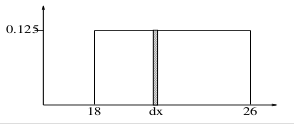
\includegraphics[width=0.5\textwidth]{chap2_pics/prop_density_function.png} 
\caption{Probability density function for equation: \ref{prop_density_func}}
\end{figure}

\subsection{Gaussian density}
\begin{theorem}[Gaussian density function]
Is a widely used density function
\begin{align}
D(X = x) = \frac{1}{\sqrt{2 \pi \sigma}}e^{-(x-\mu )^2/2\sigma^2}
\end{align}
\end{theorem}

When $\mu = 0$ the functions looks like this:\\

\begin{figure}[h]
\centering
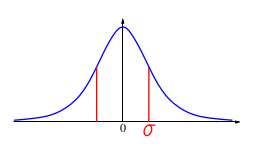
\includegraphics[width=0.5\textwidth]{chap2_pics/gausian_density_func.png} 
\end{figure}

Probability in $X \in (a,b)$ is calculated by using the \textit{probability density function} shown in equation: \ref{prop_density_func}.

\section{Proposition}
A proposition can be seen as an event(a set of sample points), where the following proposition is true:\\
\textit{A is "dice roll is less than 4"}\\

\begin{equation}
P(A) = \sum_{\omega \in A} P(\omega)
\end{equation}

Given Boolean random variables A and B:
\begin{itemize}
\item event $a$ = the set of sample points where $A(\omega)$ = true
\item event $\neg a$ = the set of sample points where $A(\omega)$ = false
\item event $a \cap b$ = points where $A(\omega)$ and $B(\omega)$ = true
\end{itemize}

Often in AI applications, the sample points are defined by the values of a set of random variables, i.e., the sample space is the Cartesian product of the ranges of the variables.\\
With Boolean variables, a sample points = propositional logic model.\\
\begin{itemize}
\item e.g. A = true, B = false, or a$\cap \neg$b
\end{itemize}

Proposition = disjunction of atomic events in which it is true.\\
\begin{table}[h]
\centering
\begin{tabular}{l l l}
$(a \cup b)$ & = & $(\neg a \cap b) \cup (a \cap \neg b) \cup (a \cap b)$ \\
$\Rightarrow P(a \cup b)$ & = & $P(\neg a \cap b) + P(a \cap \neg b) + P(a \cap b)$
\end{tabular}
\end{table}


\subsection{Inclusion - exclusion Principle}

\begin{figure}[h]\label{inclusion_exclusion_principle}
\centering
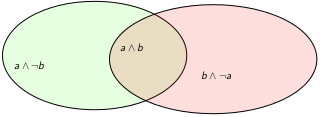
\includegraphics[width=0.6\textwidth]{chap2_pics/inclusion_exclusion.png} 
\caption{Inclusion-Exclusion Principle}
\end{figure}

The definitions imply that certain logically related events must have related probabilities(see figure \ref{inclusion_exclusion_principle}).\\
\begin{equation}
P(a \cup b) = P(a) + P(b) - P(a \cap b)
\end{equation}

\subsection{Syntax for propositions}
Propositional or Boolean random variables:\\
\begin{itemize}
\item e.g. Cavity(do I have a cavity?)
\item Cavity = \textit{true} is a proposition, also written cavity 
\end{itemize}
Discrete random variables(finite or infinite):\\
\begin{itemize}
\item e.g., Weather is one of \textit{<sunny, rain, cloudy, snow>}
\item Weather = \textit{rain} is a proposition
\item Values must be exhaustive and mutually exclusive
\end{itemize}
Continuous random variables(bounded or unbounded):\\
\begin{itemize}
\item e.g., Temp = 21.6
\item also allow, e.g. Temp < 22.0
\end{itemize}

